\begin{sloppypar}
Data has grown exponentially in the last decade and is abundantly available in various formats. Data can be categorized into structured and unstructured data. There is an abundance of structured knowledge sources available. The most prominent of which are knowledge graphs. Knowledge Graphs (KG) represent a collection of interlinked descriptions of entities, objects, events, or concepts. They put data in context via linking and semantic metadata and provide a framework for data integration, unification, analytics and sharing\cite{article}. They span many domains and are large in size. Examples of various steadily evolving cross-domain KGs include: Wikidata\cite{wikidata}, DBpedia\cite{dbpedia} and YAGO\cite{yago}  and domain specific KGs include: DrugBank\footnote{https://go.drugbank.com/} (healthcare), FoodKG\cite{foodkg} (Food Recommendation), and SoftwareKG\footnote{https://data.gesis.org/softwarekg/} (software used in science). Researchers seek effective approaches to access valuable information from these knowledge graphs as they (KG) are: i) rich in facts, ii) stored in structured databases, iii) constantly growing, and  iv) publicly available. Knowledge graphs are excellent sources of information to answer questions. But most knowledge graphs today, cover only specific domains. A knowledge graph is often represented in form of (subject, relation, object)-triples. Figure \ref{fig:kgexample} shows an example of a knowledge graph for the entity, \textbf{dbr\footnote{dbr is the prefix of http://dbpedia.org/resource/}:Steve\_Jobs}. The entity is connected to entities \textbf{dbr:The\_Walt\_Disney\_Company} and \textbf{dbr:Lauren\_Powell\_Jobs} through the relation \textbf{dbo\footnote{dbo is the prefix of http://dbpedia.org/ontology/}:board} and \textbf{dbo:spouse} respectively.
\begin{figure}
    \centering
   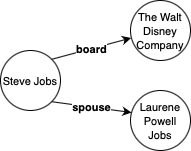
\includegraphics[width=7cm, height=4cm]{chapters/figures/SJ.png}
    \caption{An example knowledge graph}
    \label{fig:kgexample}
\end{figure}

A novice user needs to acquire both knowledge about the underlying ontology structure and proficiency in formulating formal queries (e.g., SPARQL queries) to retrieve information from Linked Data sources. To express the information in terms of SPARQL queries, users have to (a) understand the SPARQL concepts, (b) understand the SPARQL syntax (in absence of a visual query builder) and (c) know what information structures are actually available in order to formulate queries that also return results\cite{sparql}. But this limits the potential of using KGs as information sources to power-users. Therefore, approaches that rely on natural language to describe the information needs of non-expert users have been developed. These systems are called Question Answering (QA) systems.

\section{Question Answering Systems}
Question Answering over knowledge graphs is a difficult and challenging problem that has become popular in recent years. This is mainly due to the intrinsic ambiguity of natural language. Large-scale knowledge graphs such as Wikidata, DBpedia and YAGO have become important resources to solve QA problems. 

For a question answering system to understand a natural language question, it needs to: \begin{enumerate}
\item Identify entities in the question and link them to the corresponding entities in the knowledge graph.  It is a vital
component for a variety of applications built on
knowledge graphs. This involves the two sub-tasks, i.e. Named Entity Recognition (NER) and Disambiguation (NED) tasks. For instance, an ideal NED tool on DBpedia recognizes the entities embedded in the question \textit{"Who is the host of the BBC Wildlife Specials?"} and links them to the corresponding DBpedia entity (e.g., "BBC Wildlife Specials" to
\textbf{BBC\_Wildlife\_Specials}). 

\item Identify relations in the question and map them to the corresponding relations in the knowledge graph. This involves extracting the relations first and then mapping it to the correct relation in the knowledge graph. \textit{Relation Mapping} is about linking surface forms in text representing a relation to equivalent relations (predicates) of a KG\cite{falcon}. In our example question, an ideal relation mapping tool links "host" to \textbf{presenter}.

\item Build a structured representation that connects the entities and relations in the question. Following the step of understanding the question, the question answering system then finds matches between this structured representation and similar structures in the knowledge graph to find answers. 
\end{enumerate}

The focus of this thesis is on \textbf{relation mapping} because it is the most challenging out of the three steps. There has been a lot of work in the literature on entity recognition \cite{chen_shen_huang_wang_2021, OpenTapioca, Weichselbraun, tagme} in comparison with relation mapping. This has been evident if we compare the quality of recent state-of-the-art approaches \cite{falcon2, falcon}. The third step - formulating queries, depends heavily on the previous two steps and usually yields good results if the quality of the output of the first two steps (entity linking and relation mapping) is good. A system that strikes a balance between completely automatic approaches and writing complex queries is an interactive one. Therefore, there is a demand for flexible and collaborative systems to understand users and how systems can be designed to support their tasks. Interactive systems are capable of easing the understanding of a complex system and can be projected and used by inexperienced users across various domains. 

\section{Challenges in Relation Mapping}
Relation mapping faces the following challenges:  
\begin{enumerate}                                               
\item A root word can be represented in multiple ways in a KG making relation mapping difficult. Consider the question, \textbf{Who created Batman?}, the expected relation is \textbf{creator}. Both \textit{created} and \textit{creator} are derived from the root word \textbf{create}.
\item There is a comprehensive lexical gap between the words in the question and how they are represented in the KG, which makes relation mapping challenging. For example, the question \textbf{Who was the first to climb Mount Everest?} does not explicitly mention any reference to the relation \textbf{firstAscentPerson} which is the required relation to form the SPARQL query that can retrieve the answer. 
\item  Some questions need multiple relations to be linked to the target entities to get the correct answer. For instance, \textbf{Give me all cars that are produced in Germany.}, has a SPARQL query as follows,

\begin{quote}
{\fontfamily{qcs}\selectfont SELECT DISTINCT ?uri WHERE \{}
\begin{quote}
\setstretch{1.25}
{\fontfamily{qcs}\selectfont
?uri rdf\footnote{rdf is the prefix of http://www.w3.org/1999/02/22-rdf-syntax-ns\#/}:type \textbf{dbo:Automobile}. \\ \{?uri \textbf{dbo:assembly} res:Germany.\} UNION  \\ \{?uri \textbf{dbp\footnote{dbp is the prefix of http://dbpedia.org/property/}:assembly} res:Germany.\} UNION \\ \{\{?uri \textbf{dbo:manufacturer} ?x.\} UNION \\ \{?uri \textbf{dbp:manufacturer} ?x.\} \\ \{?x \textbf{dbo:locationCountry} res:Germany.\} UNION \\ \{?x \textbf{dbo:location} res:Germany.\}
} 
\end{quote}
{\fontfamily{qcs}\selectfont\}\}}
\end{quote}

This query links to the following relations \textbf{dbo:Automobile, dbo:assembly, dbp:assembly, dbo:manufacturer, dbp:manufacturer, dbo:locationCountry and dbo:location}. The SPARQL query also considers \textbf{dbo:} and \textbf{dbp:} as separate prefixes for relations. In order to get the correct answer, the user needs to know all the above relations to construct a valid SPARQL query.
\end{enumerate}

Several relation mapping tools differ based on the composition of the dataset, the training data, and the complexity of the questions \cite{4}. Most tools are geared towards string similarity and word embedding techniques. In string matching-based similarity analysis, two major similarity indexes are encountered: syntactic similarity and semantic similarity. The syntactic similarity is based on the idea that the degree of similarity between the two texts is proportional to the number of identical words in them. On the other hand, semantic similarity focuses on the meaning and interpretation between the two texts. Semantic similarity methods usually give a ranking or percentage of similarity between the texts, rather than a binary decision as similar or not similar \cite{Chandrasekaran_2022}.
For example, consider two sentences \textit{"John and Mary studied English and Science."} and \textit{"John studied English and Mary studied Science."}. Though these two sentences share the same words they do not convey the same meaning. Similarly, the questions \textit{"How old are you?"} and \textit{"What is your age?"} convey the same meaning, however, they do not have the same set of words.
String matching-based algorithms depend on the number of attempts, the number of character comparisons and the running time. These factors are influenced by the type of algorithm, type of data, data size and length of pattern - one or more strings found within a larger string or text \cite{5}. These algorithms fail to capture the semantic similarity of the sentences. Word embedding techniques like Word2Vec\cite{word2vec}, GloVe\cite{glove}, etc., are better at capturing the semantics of the words but fail when out of vocabulary words are used. They tend to be too specific and do not capture the semantics of the relationships between the entities in the knowledge graph accurately. For example, the question \textbf{Who painted The Storm on the Sea of Galilee?}, a word embedding approach would give relations like \textit{paint, painter,} etc., but it would not capture the relation \textbf{artist}.  

Interactive approaches for query formulation like Sapphire \cite{sapphire}, help the users iteratively construct SPARQL queries by providing auto-complete suggestions \textit{based on the queried data}. These systems require users to have a background knowledge of the entities and the relations to formulate queries with the correct data. The quality of the output of such systems relies excessively on the nature of the input data typed by the user. 

In order to overcome the above limitations, we propose an approach ReMLOFT : \textbf{Re}lation \textbf{M}apping Using \textbf{L}arge Corpus \textbf{O}f \textbf{F}ree \textbf{T}ext, that aims to solve the problem of relation mapping by interactively showing the users a list of candidate relations to choose for a subset of keywords in the question. Our approach aims at reducing the uncertainty faced by QA systems in the task of relation mapping. Suggesting a small set of candidate matches to the user helps in identifying the correct matches more accurately, while not overburdening the user with additional efforts or tasks. This approach heavily relies on using evidence from a large corpus of text to find a substantial number of example sentences. These sentences help in finding relations that can be mapped to connected entities in the knowledge graph. ReMLOFT constructs a free-text knowledge graph from Wikipedia, with entities (Wikipedia page titles) as nodes, and instead of depending on existing relations, ReMLOFT uses free-text sentences as edges. For example, a relation \textbf{ontology/spouse} has 53964 entity pairs and a relation \textbf{property/spouse} has 190949 entity pairs. The sentences extracted from these entity pairs give us meaningful evidence to map relations. 

Consider a triple $\textbf{\textless Steve\_Jobs, spouse,  Laurene\_Powell\_Jobs\textgreater}$, from DBpedia. We find a large number of sentences that relate the two entities \textit{
Steve\_Jobs and Laurene\_Powell\_Jobs } from Wikipedia.  Some of the sentences found are:
{\fontfamily{pcr}\selectfont
\begin{enumerate}
    \item In 1989 Jobs first met his future \textit{wife} Laurene Powell when he gave a lecture at the Stanford Graduate School of Business where she was a student.
    \item Jobs is \textit{married} to Laurene Powell Jobs (Abby Brammell) and has accepted Lisa (Annika Bertea) as his daughter (she now lives with them).
    \item On March 18 1991 Otogawa presided over the \textit{marriage} of Steve Jobs and Laurene Powell.
    \item Laurene Powell Jobs \textit{widow} of Steve Jobs was just behind Domingo inheriting a fortune of \$9 billion.
\end{enumerate}
}
From the above example sentences, we can gather that words in a sentence that connect entities, provide contextual knowledge about the relation between the two entities. Words like \textit{wife, marriage, married} and \textit{widow} from the above example can be used as links to the formal relationship in the knowledge graph (spouse).

We motivate our work by the fact that despite the vast popularity of relation mapping, there are limited attempts to interactive relation mapping over knowledge graphs. Most of the interactive approaches exist for query completion or query construction that help users write syntactically and semantically correct SPARQL queries without prior knowledge of the queried datasets\cite{sapphire}. Our approach aims to bridge the gap between the simple but ambiguous natural language approaches, and the difficult relation mapping problem.

\section{Contributions}
The main contributions of the thesis are as follows:
\begin{enumerate}
\item Building an interactive model for relation mapping that aids in querying data from knowledge graphs, where we provide suggested relations for selected keywords in the question for the user to choose from.

\item  Incorporating external evidence from a large corpus of text to support and guide the approaches used in relation mapping.

\item Building a dictionary of the most frequent keywords that define the context of a relation in the knowledge graph without using lexical tools.

\item Evaluating our approach on recent, most challenging benchmarks used for evaluating question answering systems.

\end{enumerate}

Our approach outperforms statistical and embedding-based relation mapping approaches with significant margins. It gives significant results for complex questions with more than one mapped relations. 

\section{Thesis Organization}
The rest of the thesis is structured as follows: Chapter 2 discusses the related work, and Chapter 3 describes our methodology. The experimental evaluation is presented in Chapter 4. The thesis concludes with Chapter 5.
\end{sloppypar}
